\section{Introduction to pin muxing}

\begin{frame}{What is pin muxing?}
  \begin{itemize}
  \item Modern SoCs (System on Chip) include more and more hardware
    blocks, many of which need to interface with the outside world
    using {\em pins}.
  \item However, the physical size of the chips remains small, and
    therefore the number of available pins is limited.
  \item For this reason, not all of the internal hardware block
    features can be exposed on the pins simultaneously.
  \item The pins are {\bf multiplexed}: they expose either the
    functionality of hardware block A {\bf or} the functionality of
    hardware block B.
  \item This {\em multiplexing} is usually software configurable.
  \end{itemize}
\end{frame}

\begin{frame}{Pin muxing diagram}
  \begin{center}
    \includegraphics[height=0.8\textheight]{slides/kernel-pinmuxing/pin-muxing-principle.pdf}
  \end{center}
\end{frame}

\begin{frame}{Pin muxing in the Linux kernel}
  \begin{itemize}
  \item Since Linux 3.2, a \code{pinctrl} subsystem has been added.
  \item This subsystem, located in \kdir{drivers/pinctrl} provides a
    generic subsystem to handle pin muxing. It offers:
    \begin{itemize}
    \item A pin muxing driver interface, to implement the system-on-chip
      specific drivers that configure the muxing.
    \item A pin muxing consumer interface, for device drivers.
    \end{itemize}
  \item Most {\em pinctrl} drivers provide a Device Tree binding, and
    the pin muxing must be described in the Device Tree.
    \begin{itemize}
    \item The exact Device Tree binding depends on each driver. Each
      binding is defined in \kdoctext{devicetree/bindings/pinctrl}.
    \end{itemize}
  \end{itemize}
\end{frame}

\begin{frame}{{\tt pinctrl} subsystem diagram}
  \begin{center}
    \includegraphics[height=0.8\textheight]{slides/kernel-pinmuxing/pinctrl-subsystem.pdf}
  \end{center}
\end{frame}

\begin{frame}[fragile]{Device Tree properties for consumer devices}
  The devices that require certains pins to be muxed will use
  the \code{pinctrl-<x>} and \code{pinctrl-names} Device Tree
  properties.
  \begin{itemize}
     \item The \code{pinctrl-0}, \code{pinctrl-1}, \code{pinctrl-<x>}
       properties link to a pin configuration for a given state of the
       device.
     \item The \code{pinctrl-names} property associates a name to each
       state. The name \code{default} is special, and is automatically
       selected by a device driver, without having to make an explicit
       {\em pinctrl} function call.
     \item See \kdoctext{devicetree/bindings/pinctrl/pinctrl-bindings.txt}
       for details.
  \end{itemize}
\end{frame}

\begin{frame}[fragile]{Device Tree properties for consumer devices - Examples}
  \begin{columns}
    \column{0.5\textwidth}
    \begin{minted}[fontsize=\footnotesize]{perl}
i2c0: i2c@11000 {
        ...
        pinctrl-0 = <&pmx_twsi0>;
        pinctrl-names = "default";
        ...
};
\end{minted}
    Most common case (\kfile{arch/arm/boot/dts/marvell/kirkwood.dtsi})
    \column{0.5\textwidth}
    \begin{minted}[fontsize=\footnotesize]{perl}
i2c0: i2c@f8014000 {
       ...
       pinctrl-names = "default", "gpio";
       pinctrl-0 = <&pinctrl_i2c0>;
       pinctrl-1 = <&pinctrl_i2c0_gpio>;
       ...
};
\end{minted}
    Case with multiple pin states (\kfile{arch/arm/boot/dts/microchip/sama5d4.dtsi})
  \end{columns}
\end{frame}

\begin{frame}{Defining pinctrl configurations}
  \begin{itemize}
  \item The different {\em pinctrl configurations} must be defined as
    child nodes of the main {\em pinctrl device} (which controls the
    muxing of pins).
  \item The configurations may be defined at:
    \begin{itemize}
    \item the SoC level (\code{.dtsi} file), for pin configurations
      that are often shared between multiple boards
    \item at the board level (\code{.dts} file) for configurations
      that are board specific.
    \end{itemize}
  \item The \code{pinctrl-<x>} property of the consumer device points
    to the pin configuration it needs through a DT {\em phandle}.
  \item The description of the configurations is specific to each {\em
      pinctrl driver}. See
    \kdoctext{devicetree/bindings/pinctrl} for the pinctrl bindings.
  \end{itemize}
\end{frame}

\begin{frame}[fragile]{Example on OMAP/AM33xx}
  \begin{columns}
    \column{0.55\textwidth}
    \begin{itemize}
      \small
    \item On OMAP/AM33xx, the \code{pinctrl-single} driver is used. It
      is common between multiple SoCs and simply allows to configure
      pins by writing a value to a register.
      \begin{itemize}
      \item In each pin configuration, a \code{pinctrl-single,pins} value
        gives a list of {\em (register, value)} pairs needed to configure
        the pins.
      \end{itemize}
    \item To know the correct values, one must use the SoC and board
      datasheets.
    \end{itemize}
    \column{0.45\textwidth}
    \begin{minted}[fontsize=\tiny]{perl}
/* Excerpt from am335x-boneblue.dts */

&am33xx_pinmux {
   ...
   i2c2_pins: pinmux_i2c2_pins {
      pinctrl-single,pins = <
         AM33XX_IOPAD(0x978, PIN_INPUT_PULLUP | MUX_MODE3)
         /* (D18) uart1_ctsn.I2C2_SDA */
         AM33XX_IOPAD(0x97c, PIN_INPUT_PULLUP | MUX_MODE3)
         /* (D17) uart1_rtsn.I2C2_SCL */
      >;
   };
};

&i2c2 {
   pinctrl-names = "default";
   pinctrl-0 = <&i2c2_pins>;

   status = "okay";
   clock-frequency = <400000>;
   ...

   pressure@76 {
      compatible = "bosch,bmp280";
      reg = <0x76>;
   };
};
    \end{minted}
  \end{columns}
\end{frame}

\begin{frame}[fragile]{Example on the Allwinner A20 SoC}
  \begin{center}
    \includegraphics[height=0.8\textheight]{slides/kernel-pinmuxing/allwinner-example.pdf}
  \end{center}
\end{frame}

\begin{frame}[fragile]{Illustration: live pin muxing configuration}
  \begin{center}
    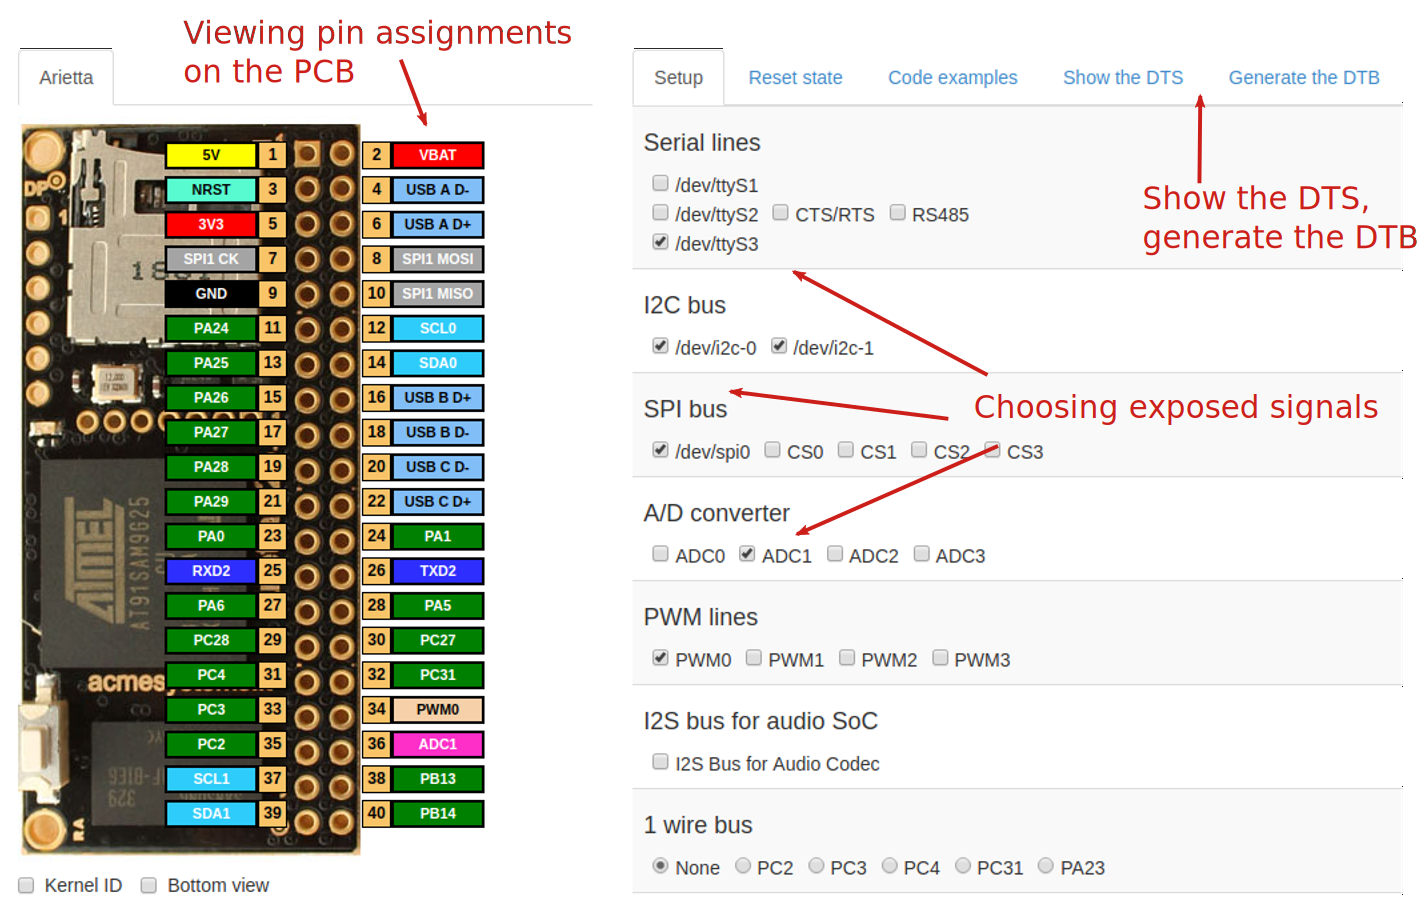
\includegraphics[height=0.7\textheight]{slides/kernel-pinmuxing/arietta-pinctrl.pdf}
  \end{center}
  Try ACME Systems' on-line pin-out generator: \url{http://linux.tanzilli.com/}
\end{frame}

\setuplabframe
{Setup pinmuxing to enable I2C communication}
{
  \begin{itemize}
  \item Configure the pinmuxing for the I2C bus used to communicate
    with the Nunchuk
  \item Validate that the I2C communication works with user space
    tools.
  \end{itemize}
}
